%% This is file `elsarticle-template-1-num.tex',
%%
%% Copyright 2009 Elsevier Ltd
%%
%% This file is part of the 'Elsarticle Bundle'.
%% ---------------------------------------------
%%
%% It may be distributed under the conditions of the LaTeX Project Public
%% License, either version 1.2 of this license or (at your option) any
%% later version.  The latest version of this license is in
%%    http://www.latex-project.org/lppl.txt
%% and version 1.2 or later is part of all distributions of LaTeX
%% version 1999/12/01 or later.
%%
%% Template article for Elsevier's document class `elsarticle'
%% with numbered style bibliographic references
%%
%% $Id: elsarticle-template-1-num.tex 149 2009-10-08 05:01:15Z rishi $
%% $URL: http://lenova.river-valley.com/svn/elsbst/trunk/elsarticle-template-1-num.tex $
%%
\documentclass[preprint,12pt]{elsarticle}

%% Use the option review to obtain double line spacing
%% \documentclass[preprint,review,12pt]{elsarticle}

%% Use the options 1p,twocolumn; 3p; 3p,twocolumn; 5p; or 5p,twocolumn
%% for a journal layout:
%% \documentclass[final,1p,times]{elsarticle}
%% \documentclass[final,1p,times,twocolumn]{elsarticle}
%% \documentclass[final,3p,times]{elsarticle}
%% \documentclass[final,3p,times,twocolumn]{elsarticle}
%% \documentclass[final,5p,times]{elsarticle}
%% \documentclass[final,5p,times,twocolumn]{elsarticle}

%% The graphicx package provides the includegraphics command.
\usepackage{graphicx}
%% The amssymb package provides various useful mathematical symbols
\usepackage{amssymb}
%% The amsthm package provides extended theorem environments
%% \usepackage{amsthm}
\usepackage{tabularx}
%% The lineno packages adds line numbers. Start line numbering with
%% \begin{linenumbers}, end it with \end{linenumbers}. Or switch it on
%% for the whole article with \linenumbers after \end{frontmatter}.
\usepackage{lineno}
\usepackage[round]{natbib}
%% natbib.sty is loaded by default. However, natbib options can be
%% provided with \biboptions{...} command. Following options are
%% valid:

%%   round  -  round parentheses are used (default)
%%   square -  square brackets are used   [option]
%%   curly  -  curly braces are used      {option}
%%   angle  -  angle brackets are used    <option>
%%   semicolon  -  multiple citations separated by semi-colon
%%   colon  - same as semicolon, an earlier confusion
%%   comma  -  separated by comma
%%   numbers-  selects numerical citations
%%   super  -  numerical citations as superscripts
%%   sort   -  sorts multiple citations according to order in ref. list
%%   sort&compress   -  like sort, but also compresses numerical citations
%%   compress - compresses without sorting
%%
%% \biboptions{comma,round}

% \biboptions{}

\journal{Hydrological Procesesses}

\begin{document}

\begin{frontmatter}

%% Title, authors and addresses

\title{Surface and subsurface runoff hydrological partitioning. The role of rainfall features and antecedent soil moisture conditions in a tropical watershed.}

%% use the tnoteref command within \title for footnotes;
%% use the tnotetext command for the associated footnote;
%% use the fnref command within \author or \address for footnotes;
%% use the fntext command for the associated footnote;
%% use the corref command within \author for corresponding author footnotes;
%% use the cortext command for the associated footnote;
%% use the ead command for the email address,
%% and the form \ead[url] for the home page:
%%
%% \title{Title\tnoteref{label1}}
%% \tnotetext[label1]{}
%% \author{Name\corref{cor1}\fnref{label2}}
%% \ead{email address}
%% \ead[url]{home page}
%% \fntext[label2]{}
%% \cortext[cor1]{}
%% \address{Address\fnref{label3}}
%% \fntext[label3]{}


%% use optional labels to link authors explicitly to addresses:
%% \author[label1,label2]{<author name>}
%% \address[label1]{<address>}
%% \address[label2]{<address>}

\author[1,2]{N. Velasquez}
\author[2]{S. Castillo}
\author[2, 3]{C.D. Hoyos}

\address[1]{Iowa University, IIHR}
\address[2]{EAFIT university.}
\address[3]{Universidad nacional de Colombia.}

\begin{abstract}
%% Text of abstract
Suspendisse potenti. Suspendisse quis sem elit, et mattis nisl. Phasellus consequat erat eu velit rhoncus non pharetra neque auctor. Phasellus eu lacus quam. Ut ipsum dolor, euismod aliquam congue sed, lobortis et orci. Mauris eget velit id arcu ultricies auctor in eget dolor. Pellentesque suscipit adipiscing sem, imperdiet laoreet dolor elementum ut. Mauris condimentum est sed velit lacinia placerat. Vestibulum ante ipsum primis in faucibus orci luctus et ultrices posuere cubilia Curae; Nullam diam metus, pharetra vitae euismod sed, placerat ultrices eros. Aliquam tincidunt dapibus venenatis. In interdum tellus nec justo accumsan aliquam. Nulla sit amet massa augue.
\end{abstract}

\begin{keyword}
Science \sep Publication \sep Complicated
%% keywords here, in the form: keyword \sep keyword

%% MSC codes here, in the form: \MSC code \sep code
%% or \MSC[2008] code \sep code (2000 is the default)

\end{keyword}

\end{frontmatter}

%%
%% Start line numbering here if you want
%%
\linenumbers

%#################################################################
%% main text
\section{Introduction}
\label{intro}

During a storm event the hydrograph is mainly formed by surface and subsurface runoff volumes \citep{Flury1994,Jackisch2016}. The separation of those runoff volumes is referred to as flow partitioning \citep{Munoz2012}. Soils, land use, topography, and external forcings such as rainfall spatio-temporal patterns, and pre-event water, modulate the surface and subsurface partition \citep{radatz2013, Shope2016}. Understanding the link between flow partitioning and external forcings is fundamental for catchment hydrology assessment and hydrological model implementation \citep{todd2006,Tetzlaff2008}.  Due to this relevance, several methods have been used to assess the characterization of flow partitioning, including field techniques \citep{Shope2016}, tracers \citep{Tetzlaff2008}, digital filters \citep{Eckhardt2005,Stewart2015a}, and modeling approximations \citep{Partington2011, Dukic2006}.  In spite of the several attempts, the large number of techniques, and the differences in the results, there is no consensus on which is the best approach to analyze forcings on runoff mechanisms during storm events (\citep{Stewart2015a, Blume2015, Penna2015}. The  high level of subjectivity still involved in such analysis indicates that the problem is not fully understood \citep{Dukic2006, Tallaksen1995}.\\

Despite the above mentioned differences, it is clear that subsurface runoff plays a crucial role during storm events \citep{Pinder1969, Sklash1979, Wels1991, Zehe2010,Blume2015, Jackisch2016}.  Evidence could be found in several cases. Using tracers in three basins of Nova Scotia, \citet{Pinder1969} found that around 40\% of the total runoff is explained by subsurface.  \citet{Eckhardt2005} obtains a similar result using digital filters,  with subsurface contribution oscillating between 25 and 80\% of the streamflow.  \citet{Shope2016} presented a similar result in the Haean-Myun catchment (South-Korea), with subsurface contributions around 46\% of the hydrograph.  There are also indirect results that reinforce the idea of a strong subsurface flow participation. Using field observations and simulations,  \citet{Sklash1979} found large and rapid increases of the hydraulic head in the near-stream groundwater after the start of the rain. \citet{Kubota1995} compared modeled results with observations, and showed that a significant portion of the streamflow is explained by subsurface runoff equations.\\ 

Subsurface stormflow portion tends to be highly variable, characteristic that rises questions regarding the processes and the interaction with forcing variables such as rainfall or pre-event water \citep{Dunkerley2017, Jackisch2016, Torch2013}.  Rainfall external forcing exhibits a high spatiotemporal variability which may impact the hydrograph partitioning.  High intense events, with low accumulation and short duration, increase surface and lower subsurface production CITA(Liu, 2016).  On the other hand, low intensity and long duration rainfall events, increase subsurface volume \citep{Rusjan2015, Blume2015}. By inducing synthetic abrupt temporal variations in the rainfall, \citep{Dunkerley2008} found significant reductions of the runoff production. The rainfall interactions variability are not limited to high or low intensities, they change also in function of the basin area, topography and soil textures \citep{Shope2016, Shope2014}. According to \citep{Mei2015a} rainfall duration increases with the basin area, and so does the subsurface production.  Also, field findings suggest rainfall features and their variability influence partitioning and the displacement of pre-event water \citep{Zabaleta2013, Penna2011}.  The mentioned results give an idea about the role of the rainfall.  However, there is a lack of evidence that links rainfall spatio-temporal variability with the dynamic of the stormflow partitioning \cite{Gomi2010}.\\

In addition to rainfall, pre-event water also plays a crucial role on the stormflow partitioning variability \citep{Dusek2016, Klaus2013,Clow2000,Sklash1979}. Although subsurface runoff could be different from pre-event water, both variables are highly correlated \citep{Wels1991, Rusjan2015}. Using isotopes, \citet{Sklash1979} showed that pre-event water dominated the hydrograph in humid systems.  In another humid watershed, \citet{Cey1998} found that pre-event water explains the 80\% of the hydrograph.  A comparable value was reported by \citet{Buda2009} for a 45$km^2$ catchment.  Bazemore (1994) observed that pre-event water increases contribution to the transient saturated zone during storm events.  In a small catchment, \citet{Dewalle1994} reported a pre-event water participation between 55 and 94\%.  Similar values were reported by \citet{Carey2005} with pre-event water ratios above 50\%. In a small catchment (0.198$km^2$). \citet{Munyaneza2012} reported pre-event water contributions of 60 and 80\% for catchments with areas of 129 and 257.4$km^2$ respectively.  Additionally, the participation and influence of pre-event water on the hydrograph partitioning could be partially conditioned by the rainfall variability \citet{Clow2000}.\\  

In the present work, we want to explore how the variability of both forcings (rainfall and pre-event water) and their interplay influence stormflow partitioning. Using a modeling approach, we analyze rainfall and pre-event water interactions on the hydrograph partitioning in a tropical catchment. We use the distributed hydrological model WMF (Watershed Modeling Framework) \citep{Frances2007}, with the ability to separate surface and subsurface runoff.  Rainfall is derived from a C-band weather radar, model calibration and validation is achieved with a stage station data located at basin outlet. Pre-event water is analyzed from model states obtained with an hourly scale simulation achieved for reccords between 2013-2017. Then, stormflow partition is analyzed for each event simulated at a 5min time step for each event, simulations at 5 min. scale is carried out and stormflow partition is analyzed for each event using at a 5 min time step simulation. Variability of simple features such as maximum intensity and total stored volume are contrasted against the flow partitioning. The experiment was conducted with 128 storm events to get conclusive results about the catchment response under storm events.\\

%#################################################################
%% main text
\section{Data and methods}
\label{methods}
We present the overall methodology followed in the present work in an illustrative diagram in Figure 2.  For the experiment, we made a mid-term simulation with the distributed hydrological model at a time step of one hour for the period between 2013 and 2017.  In this same period, we did simulate 128 storm events with the conditions obtained from the mid-term simulation.  For each event, the model separates surface and subsurface runoff, which was then compared against rainfall and pre-event water features. The rainfall features include intensity, depth, and days since the last storm.  On the other hand, soil conditions features include the mean gravitational storage from three hours before each storm event, and the time passed since the last storm event.\\

\subsection{Study and area}

The current work is done in the Valle de Aburrá (VA) watershed, located on the north-east part of Central Colombian Andes (see Figure \ref{fig:localization}).  In the region, there is a high frequency of local convective cores which produce intense storm events \citep{Zuluaga2015}. This fact along with locally steep slopes and the urbanization of the watershed (24\% of the total area), produces abrupt changes in the streamflow during storm events. Also, there are human settlements near steep network tributaries subject to abrupt changes.  The mentioned characteristics give hydrological and political relevance to the analysis of the hydrograph formation during storm events. 

Several information resources were used to develop the analysis.  ALOS-PALSAR elevation raster data \citep{ALOS} was used for the basin delineation and also for the estimation of the distributed geomorphological parameters.  From POMCA (a local environmental project of the watershed) we obtained land use, roughness and soil information. Soils hydraulic properties were derived from the soils texture descriptions by using the SPAW software \citep{Saxton2006}.

\begin{figure}[t]
    \centering
    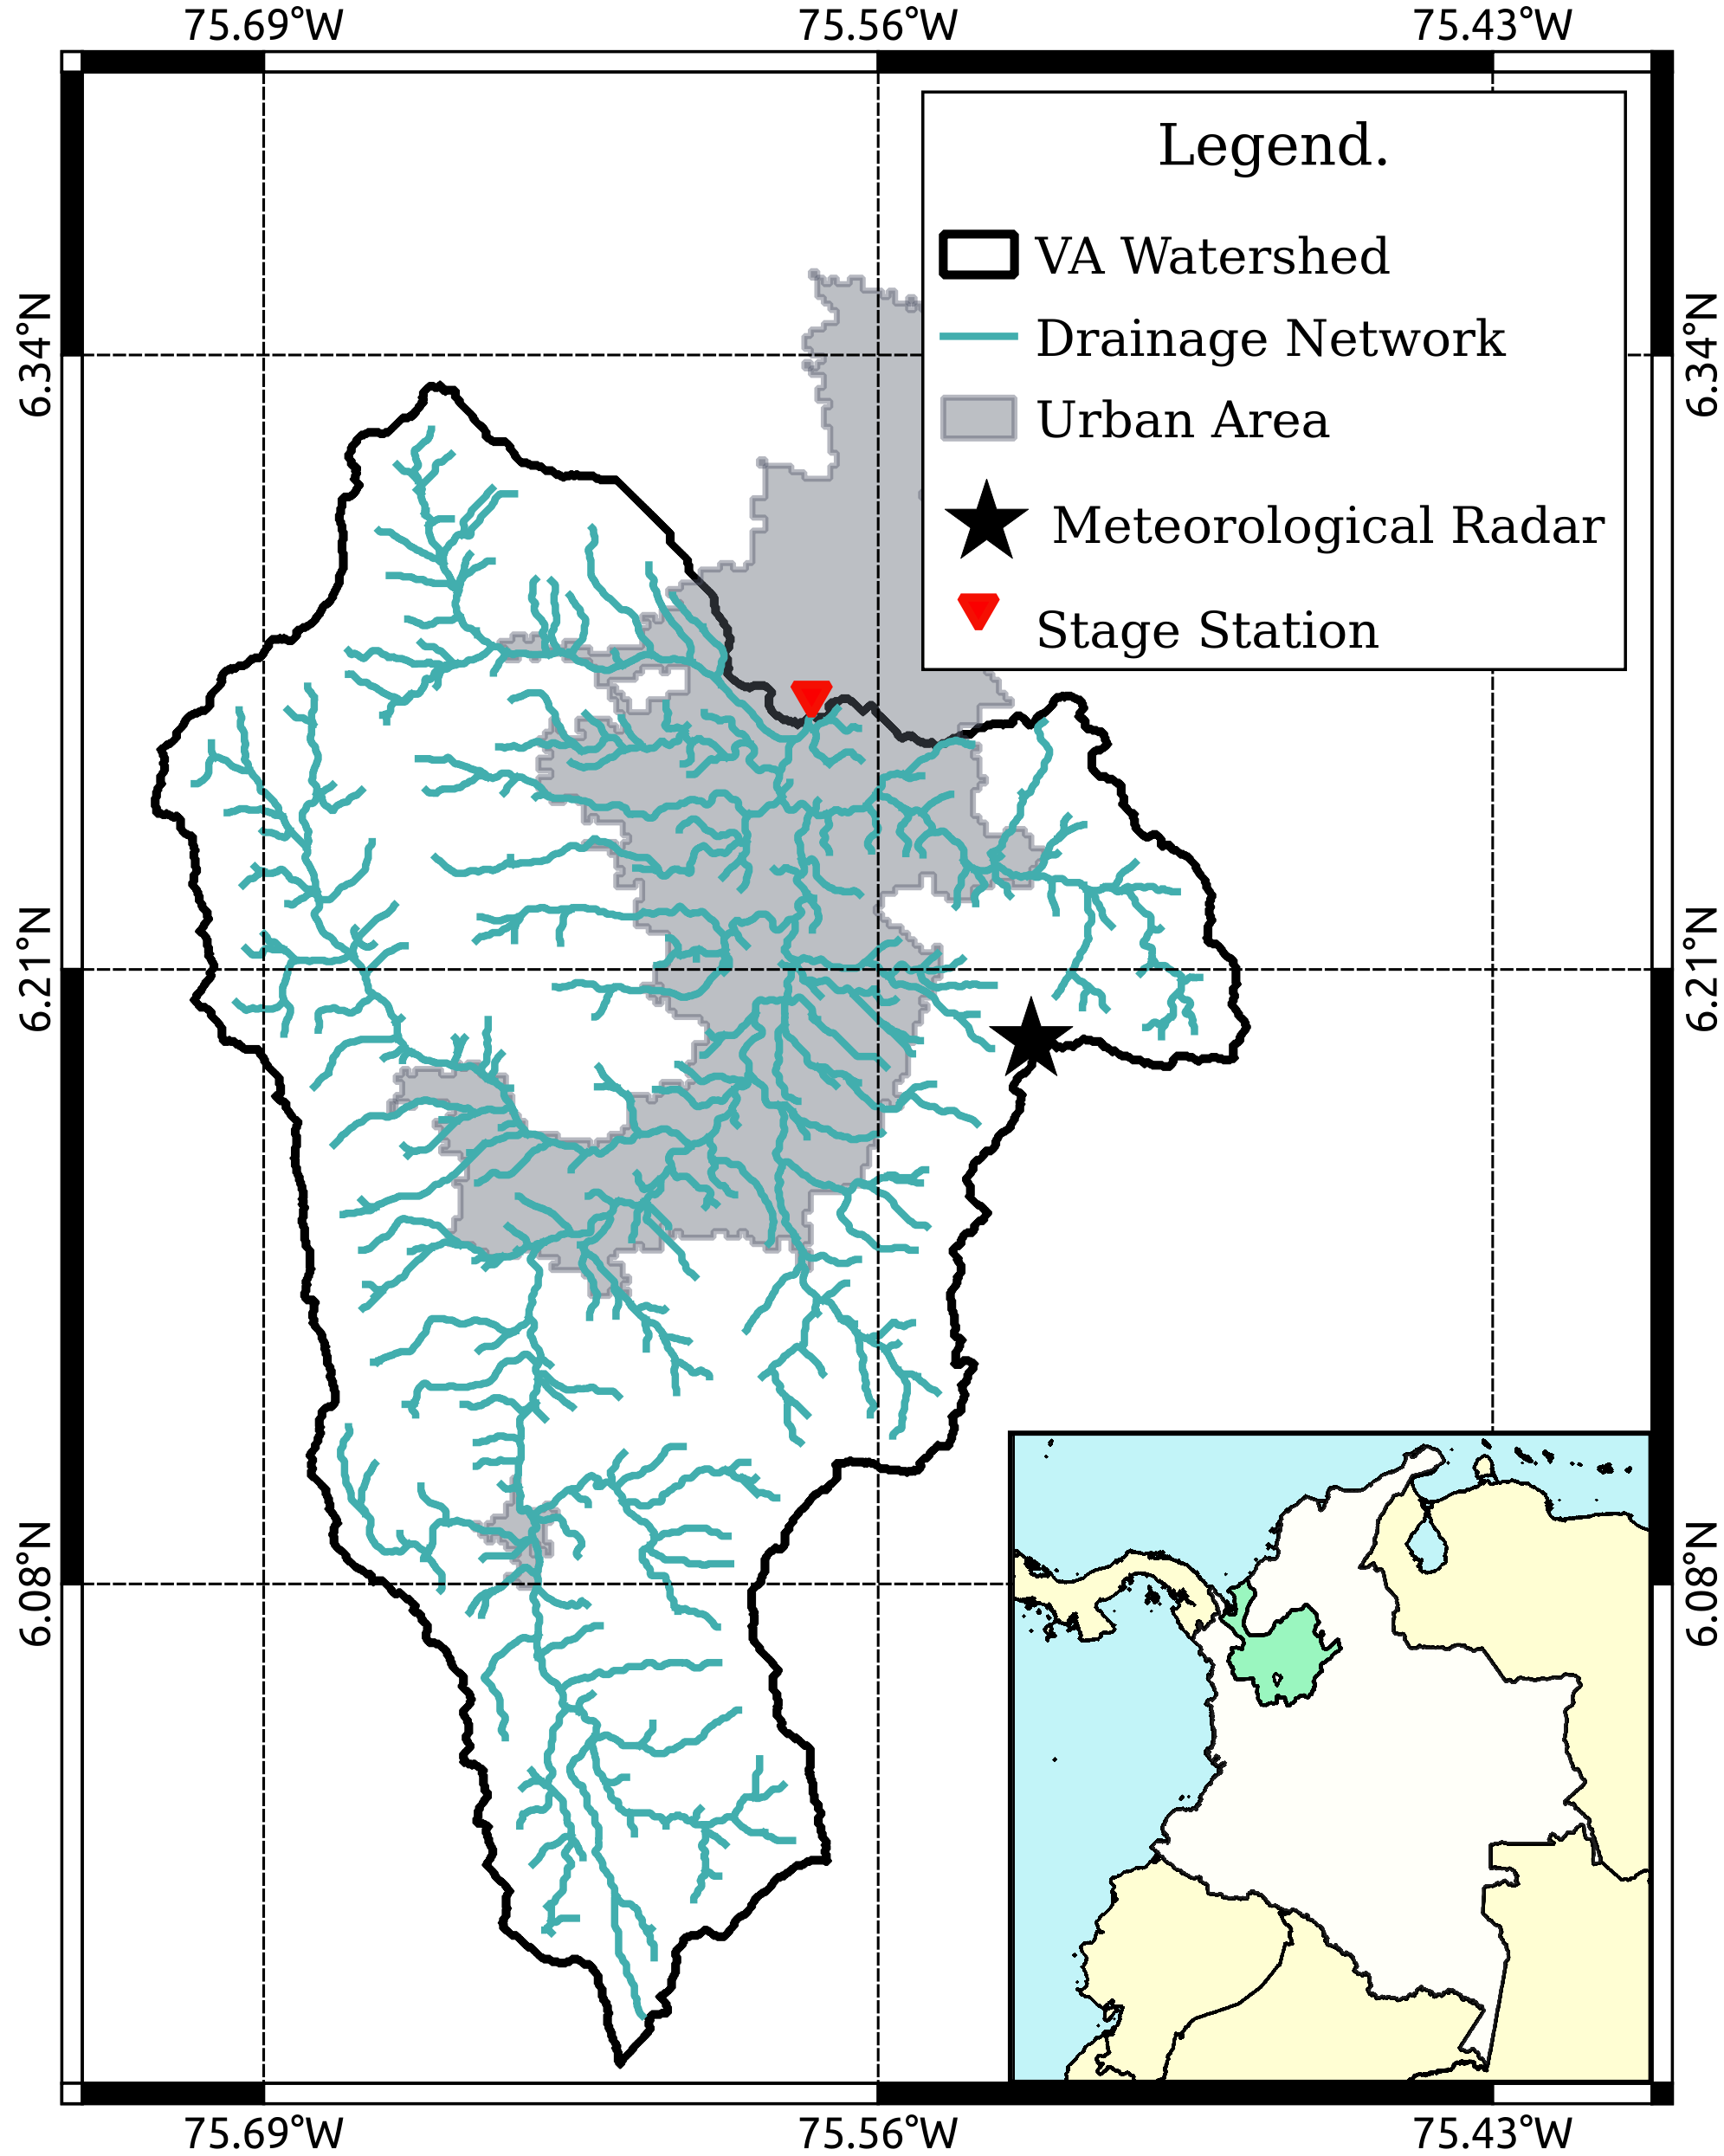
\includegraphics[width=8.3cm]{Figuras/layout_aula3.png}
    \caption{Watershed, radar and stream gauge localization.}
    \label{fig:localization}
\end{figure}

VA is a typical tropical mountainous basin with variable topographical and soil textures. The main channel presents a mean slope of 1.83\%, it starts at approximately 2300 masl, while the outlet is around 1400 masl (884 m of height gradient). In contrast, some sub-basins show height differences of 2000$m$. The mean basin slope is about 30\%, with some hills reaching values between 50\% and 80\%.  Soils are mainly composed of sand and silt with a low percentage of clay (POMCA, 2007). Depths estimations of the soil profile (Z) oscillate between 0.2 and 1 m \citep{Osorio2008}, being deeper at the foothills than at the slopes development. Hydraulic conductivity (Ks) varies between 10 and 125 mm/h, with higher values on the hills in the south-west.  The hydraulic properties of the soils led to the estimation of the capillary ($H_u$) and gravitational ($H_g$) storage capacity. $H_u$ oscillates between 20 and 200 $mm$ and $H_g$ between 15 and 500$mm$.\\

Used temporal information includes a local level station located at the outlet of the basin (red triangle at Figure \ref{fig:localization}) and QPE estimations from a meteorological radar.  The level information dates from 2011 to 2018 with a time step of 1min.  The QPE technique was developed by Sepúlveda and Hoyos (2018).  This technique uses retrievals from a C-band polarimetric Doppler weather radar operated by the Sistema de Alertas Tempranas de Medellín y del Valle de Aburra (SIATA).  The quality of the radar data is high due to its vicinity to the basin (black star at Figure \ref{fig:localization}), however, the radar does not detect information in its immediate vicinity (blue circle in Figure \ref{fig:localizacion}).  Due to the operating strategy of the radar the information is collected every 5$min$ at a spatial resolution of 128 $m$.\\

Temporal information consists of a stage station located at the basin outlet and the mentioned QPE estimations; both records were obtained by the local early warning system (Sistema de Alerta Temprana de Medellín y el Valle de Aburrá, SIATA). The stage station is over the main channel; it counts with several streamflow measurements which lead to a robust rating curve.\\

\subsection{Hydrological model and flow separation }

For the hydrological simulation, we use a modification of the distributed hydrological model proposed by \citep{Frances2007, Velez2001}.  The model discretizes the watershed into cells, for this case we use a resolution of 30x30m.   In each cell, five tanks represent the hydrological storages: capillary (tank 1), gravitational (tank 2), runoff (tank 3), baseflow (tank 4) and streamflow  (tank 5).  The state of each tank ($S_i$) varies in function of the vertical and lateral flows as shown in Figure 2,  $S_i$ varies in function of its inputs ($D_i$) and outputs ($E_i$). The value of $D_i$ oscillates in function of the vertical inflow ($R_i$) and the vertical interaction with its surrounding tanks.  For tank 1, the input is represented by the rainfall at the cell ($R_1$) and the output $E_1$ corresponds to the evaporated water, in the remaining tanks $E_i$ corresponds to a horizontal outflow. 

Based on two threshold accumulated areas, the model classifies the watershed into three types of cells: hill cells, cells with ephemeral streams, and cells with perennial streams.  The connection between tanks and cells varies in relation to the types of cells.  At hill cells, $E_i$ goes to the same tank of the downstream cell.  At ephemeral cells,$E_2$ and $E_3$ go to tank 5 and $E_4$ goes to the cell downstream. In the perennial cells, $E_2$, $E_3$ and $E_4$ go to tank 5.  $E_5$ goes downstream for both ephemeral and perennial streams.  At tanks 2, 3 and 5 the lateral flow $E_i$ is approximated by a kinematic equation.  Surface runoff speed ($E_2$) is explained by a modification of Manning's formula for flow in gullies \citep{Foster1984} (equation \ref{eq:foster}).  Subsurface runoff ($E_3$) is explained by the \citep{Kubota1995} approximation (equation \ref{eq:kubota}).  The subterranean flow ($E_4$) is assumed as a linear tank. And, the Geomorphologic Kinematic Wave approximation \citep{Velez2001} is used to estimate the channel flow ($E_5$) speed.  More information on the model could be found at \citep{Velez2001, Frances2007}. \\

\begin{equation}
 v_{2} = \frac{\varepsilon}{n}  S_{0}^{1/2} A_{2}(t)^{(2/3) e_1}
    \label{eq:foster}
\end{equation}

\begin{equation}
 v_3 = \frac{K_s S_{o}^{2}}{(b+1) A_{g}^{b}} A_{3}(t)^{b}
    \label{eq:kubota}
\end{equation}

\begin{equation}
 v_4 = \Omega A_4^{\omega_1} S_0^{\omega_2} \Lambda^{\omega_3} 
    \label{eq:ocg}
\end{equation}

In addition to the hydrological processes, the model can track surface (tank 2) and subsurface (tank 3) streamflow contribution at each channel reach. It marks water once it reaches any of those two tanks, and the surface-subsurface flow percentage is taken into account once the water enters tank 5 (the channel).   At this point, the model assumes that the water in the channel is well mixed,  implying that the surface and subsurface portions are constant until a new inflow enters the channel.  It is important to notice that this estimation does not interfere with the calculation of the flow process downstream.\\ 

\subsection{Experiment set}

We parametrize and validate the model for a mid-term simulation with an hourly time step, and also at event-scale (5min).  For this, we used the radar and streamflow registers between 2013 and 2017.  At each time step, we saved the states of the mid-term model which were then used as the initial conditions for the event simulations.  The streamflow partitioning only works over the events simulated at 5min scale.\\

The primary goal of the present work is to analyze how rainfall and pre-event soil water influence surface and subsurface partitioning during storm events.  With this regard, we perform a qualitative evaluation of four selected events and a quantitative analysis including all the cases (128).  The qualitative analysis considers the spatiotemporal variations of the observed rainfall.  For the quantitative analysis, we analyze two main features of the rainfall: the maximum mean intensity ($I_{max}$), and the total rainfall depth ($P_{tot}$).  $I_{max}$ is obtained directly from the rainfall hietogram, which is obtained at each time step $t$ as the mean intensity observed by the radar, and $P_{tot}$ is the sum of the hietogram at the end of the event.  For this analysis we also consider the model soil storage ($S_3$), and the dry hours before each event ($T_{dry}$) as proxies of the pre-event soil water for each event.   Finally, we compared the mentioned variables against the hydrograph volume partitioned by the model as $V_{sur}$ (surface runoff volume) and $V_{sub}$ (subsurface runoff volume).  In some figures, both variables appear as a percentage of the total streamflow volume.\\

%#################################################################
%% main text
\section{Results and Analysis}
\label{results}

The model performance was evaluated at a mid-term scale (hourly) and at an event scale (5min) for each one of the N events.  There is an overall good performance of the model in the mid-term simulation (NE value of XX and Figure 4), which gave us confidence about the initial conditions for the event scale simulations. In the event scale, the model starts the simulation 3 hours before the peak-flow and ends 3 hours after.  For a more comprehensive analysis, four events were analyzed in detail, considering spatiotemporal variations of the rainfall by a qualitative analysis of the radar fields.  Complementary, we analyzed streamflow partitioning variability of all events involving the total partitioned volume, rainfall features, and pre-event conditions.  Results show that streamflow partitioning depends on pre-event water, rainfall variability, and their interplay.\\      

\subsection{Parameterization and validation}

In the parametrization process, we search for scalar values corresponding to each physical variable of the model \citep{Frances2007}.  The search ends when the model simulated streamflow fits the observed streamflow at the outlet (red station at Figure \ref{fig:localization}).  At Table \ref{tab:parameters} we show the obtained parameters for the hourly and 5min simulations.  At both scales, the values of $H_u$ and $H_g$ are equal. Moreover, the most sensitive parameters correspond to the subsurface hydraulic conductivity ($K_s$), deep conductivity ($K_p$), surface flow velocity ($V_1$) and subsurface flow velocity ($V_2$).\\

\begin{table}[]
        \centering
        \begin{tabularx}{\textwidth}{p{3cm} p{2.2cm} p{1.5cm} p{2cm} p{3.5cm}}
\hline
Parameter Name & Symbol & Long term & Event & Spatial distribution \\
\hline
Capilary storge & Hu [mm] & 1 & 39 & In function of the slope \\
Gravitational storage & Hg [mm] & 1 & 34 & As a function of the slope \\
Evaporation rate & Etr [mm/s] & 0.1 & 0.01 & As a function of the DEM \\
Infiltration rate & ks [mm/s] & 2.7 & 0.0012 & Lumped \\
Percolation rate & kp [mm/s] & 0.8 & 0.00012 & Lumped \\
System losess & Kf [mm/s] & 0 & 0.0 & Lumped \\
Surface speed & vr [m/s] & 0.5 & 6.4 & As a function of the slope and storage \\
Subsurface speed & vs [m/s] & 1 & 7.1 & As a function of the slope, Hg and storage\\
Subterranean speed & vb [m/s] & 0.5 & 0.000095 & Lumped \\
Channel speed & vc [m/s] & 1 & 0.95 & As a function of the slope, acumulated area, and storage \\
\hline
\end{tabularx}
        \caption{Hydrologic model parameters.}
        \label{tab:parameters}
    \end{table}

The results shows that the model has an overall acceptable performance.  At an hourly scale, the model achieves an $NE$ value of 0.3 which is an acceptable performance considering that it is out of the focus of the present work.  At the event scale, the performance considers $NE$, $QmaxDif$ (peak streamflow difference), and $VtotDif$ (total volume difference).  For 40\% of the events the model gets $NE$ values above 0.6, $50\%$ with $NE$ values above 0.4, and $QmaxDIf$ values below XX, a distribution of the event-scale performance is shown in Figure \ref{fig:performance}.  Considering that poor performance events could bias our analysis, we only consider events with $NE$ values above 0.4.\\

\begin{figure}[t]
    \centering
    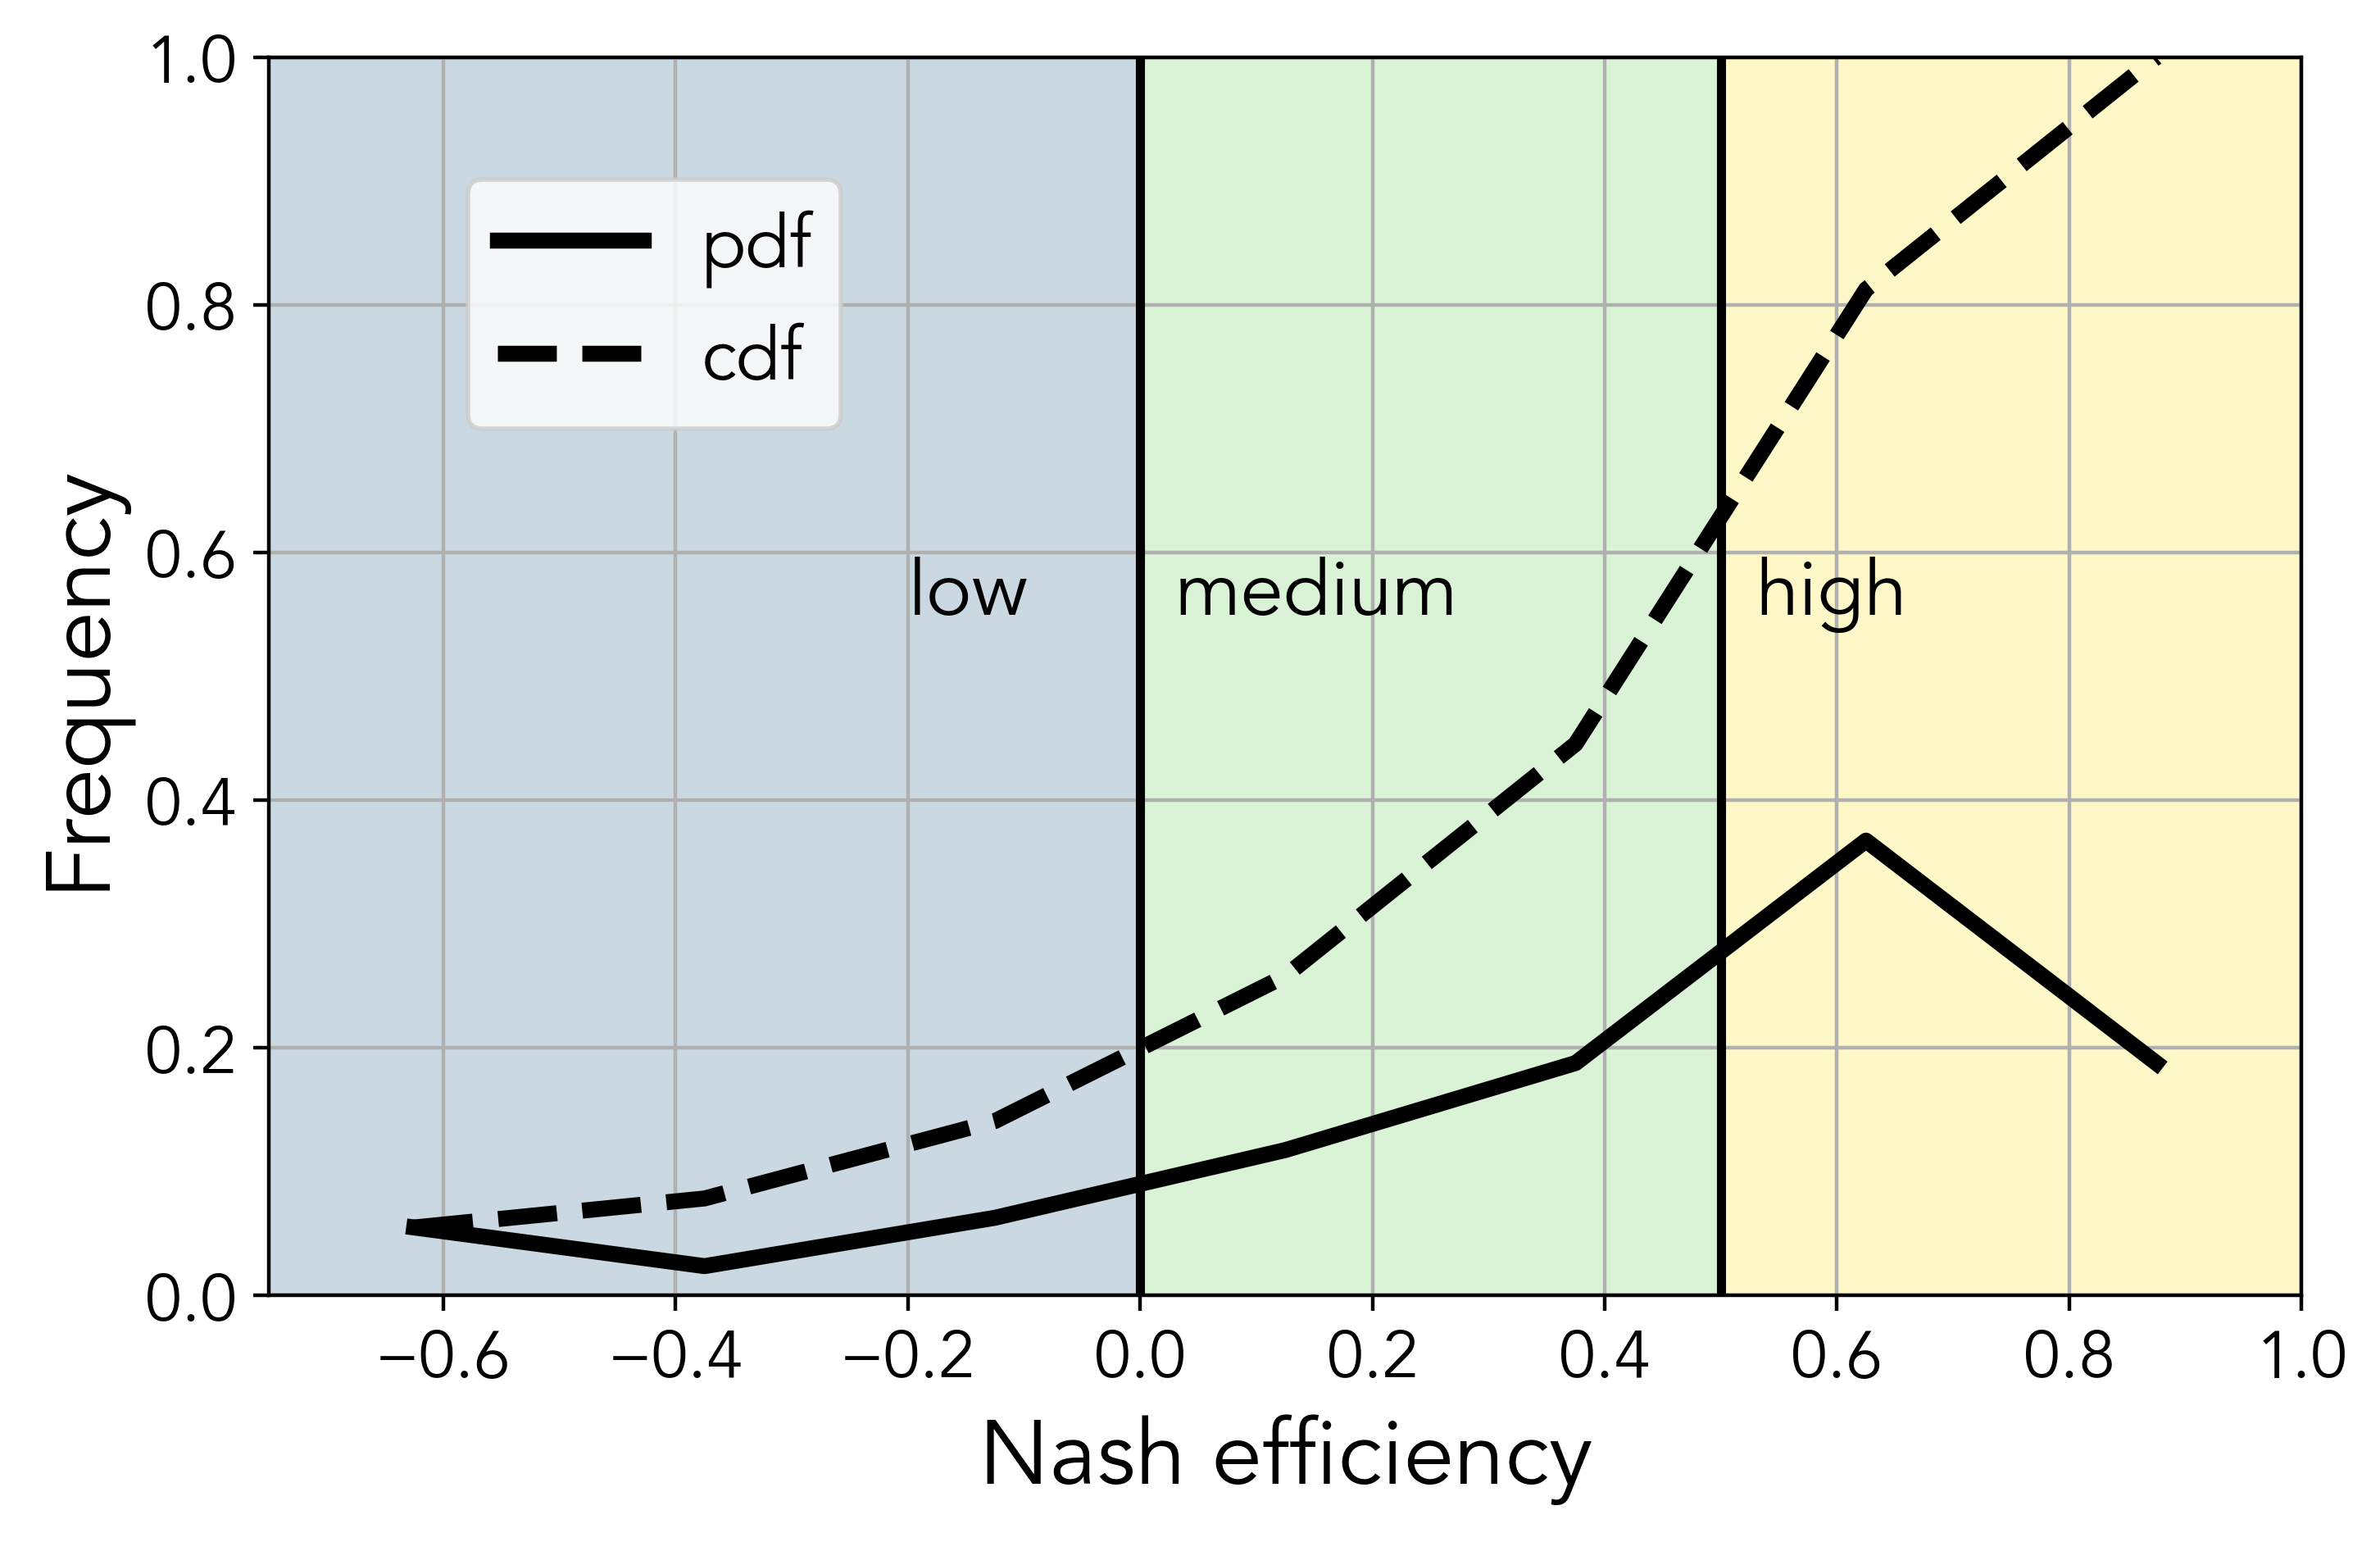
\includegraphics[width=8.3cm]{Figuras/PerformNS_pdf.png}
    \caption{Nash sutcliffe performance distribution for the analyzed events.}
    \label{fig:performance}
\end{figure}

\subsection{Stormflow partitioning at 4 specific cases}

We first analyze 4 events in detail in order to assess how variations at rainfall and soil moisture condition the streamflow partitioning. The four events were selected by their variations on the total percentage of surface and subsurface runoff.  According to this, there are two well mixed events, one surface dominated event and a subsurface dominated one (Figure 3). For the analysis, we took into account the hietogram evolution, rainfall spatial accumulation, pre-event water, and radar profiles at different time steps.\\

In addition to the volume partitioning, there are several differences between the four selected events (Figure \ref{fig:four_events}).  At events E5 and E100 there is a maximum rainfall accumulation of 0.8 and 0.85 $mm$ in 5min (9.6 and 10.2 $mm/h$ respectively), in events E120 and E186, this accumulation descends to 0.45 and 0.2 respectively.   Also, there are differences regarding the temporal distribution of the rainfall.  At events E5 and E100 the major accumulation happens in a time lapse of 1 hour,  on the other hand, for events E120 and E186, the corresponding major accumulation happens in a lapse of  3 hours respectively.\\

Described differences in the rainfall influence the observed streamflow and the simulated partitioning.  In the four cases, peak streamflow and flow partitioning vary in function of the hietogram evolution.  Surface runoff increases with the mean maximum intensity, and subsurface runoff with low-intensity and long-duration rainfall events as shown on event E186 (Figure \ref{fig:four_events}).\\

\begin{figure}[t]
    \centering
    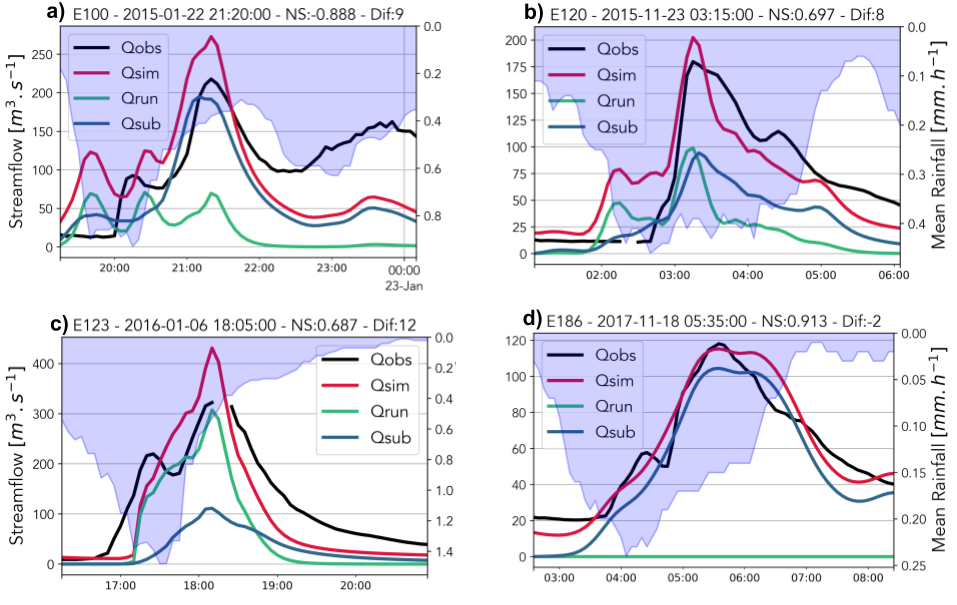
\includegraphics[width=14cm]{Figuras/Cuatro_eventos.png}
    \caption{Selected stormflow events, in each event we present the observed streamflow (black), total simulated streamflow (red), simulated surface runoff (green) and simulated subsurface runoff (blue), also we show rainfall depth in an inverted second y-axis. E100 and E120 are well mixed events between surface and subsurface. E123 is a surface runoff dominated event, and E186 is a subsurface dominated event.}
    \label{fig:four_events}
\end{figure}

The accumulation of the rainfall fields during the events also plays a relevant role on the partitioning dynamics (Figure 4).  With high intensities and more surface runoff, events E5 and E120 exhibit high rainfall accumulation in a limited spatial domain.  Conversely, the rainfall field accumulation is almost homogeneous at the subsurface dominated event E186.   Finally, event E100 has a mix between regions with homogeneous low rainfall accumulation and sparse regions with medium to high accumulations (Figure 4b) which correspod to two peaks at the hietogram and temporal oscillations in the flow partitioning (Figure 3b).\\

FIGURE RAINFALL ACCUMULATION

\subsection{Stormflow partitioning in function of rainfall and pre-event conditions.}

As presented from the four analyzed events, rainfall and initial conditions do influence streamflow partitioning.  A similar behavior is observed when we analyze all the storm events recorded between 2014 and 2017.   Figures 5 and 6 show the results obtained when we observe subsurface and surface total partitioned volumes in function of rainfall features and pre-event conditions.\\  

Total rainfall and mean maximum intensity are indirectly interrelated (Figures 5a and b) and both partially influence stormflow partitioning.  Subsurface runoff and surface runoff increase with the total rainfall and the intensity respectively.  Despite this, partitioning variability is not fully explained by this rainfall features.  In Figure 5a there are cases with medium-high values of total rainfall and high surface runoff volume. A similar case is present in Figure 5b where subsurface runoff predominates for some mid intensity events.\\

FIGURE 5. Subsurface vs surface partitioned volume compared against a) the total rainfall of each event and b) the maximum mean intensity of each event.\\

Pre-event conditions of the soils also play a role in the partitioning.  Figure 6 presents the partitioned volume in function of the elapsed time from the last storm and the simulated mean storage one day before each event.  Surface runoff increases with the elapsed time from the last storm event, and with the decrease of the mean storage.  On the other hand, subsurface runoff increases when there is more mean storage and less elapsed time from the last storm. The described results could be linked to the absence or presence of old water that goes out as subsurface runoff (CITAS), but this is a hypothesis that must be tested.\\

FIGURE 6. Subsurface vs surface partitioned volume compared against a) time from the last strom b) mean storage the day after the event.\\

In Figure 7 we remark the differences that appear when there is a change of the independent variables (rainfall features or soil pre-event conditions).  According to Figure 7, streamflow partitioning behaves differently with respect to each variable.  Due to hortonian runoff production, maximum intensity increases surface volume and has a poor effect over the subsurface runoff evolution (Figure 7a).  On the other hand, total rainfall and subsurface increase simultaneously, with little effect over the surface runoff.\\

Figure 7c and d show the results for the streamflow partitioning compared to the mean soil storage the day before the event, and the elapsed time since the last storm event. Figure 7c shows that the increase in the mean storage has a poor effect over the flow partitioning. On the other hand, high values of subsurface runoff volume correspond to low values of elapsed time since the last storm.  Nevertheless, the elapsed time seems to have no effect over the surface runoff volume.\\

FIGURE 7. Flow partitioning evolution in function of the mean maximum intensity (a), the accumulated rainfall (b), the mean storage of the the basin one day before (c) and the elapsed time from the last storm (d).\\

To finish this analysis, in Figure 8 we compare surface and subsurface runoff to maximum intensity by using colors to identify the mean storage of each event.  At Figure 8a we can see that low values of subsurface runoff correspond to high values of maximum intensity, and this relation tends to be limited for cases with low mean storage values.  On the other hand, low-intensity values increase subsurface runoff volume, and this tends to happen more often for high values of the mean storage.  As presented at Figures 6a and 7a, the maximum intensity is directly related to the surface runoff production, with no relevant relationship with the soil mean storage.\\

FIGURE: Variación del volumen surface y subsurface en funcón de la intensidad y el almacenamiento medio.\\

\section{Conclusions}

By using a hydrological model, we perform a conceptual evaluation of the surface and subsurface flow partitioning. We conduct a qualitative and quantitative analysis of the model results.  The qualitative analysis consists of the evaluation of four selected events (FIGURE), for which we describe the overall results with graphics of the hydrographs, and the spatiotemporal rainfall distribution.  On the other hand, in the quantitative analysis we include all the storm events recorded between 2012 and 2017.  For this case, we compare the results from the partitioning process with key features of the rainfall and the soil moisture of the watershed.  At least in this conceptual approximation, our results highlight the variability of the flow partitioning, and its dependence on some processes.\\

The qualitative analysis of the selected four events, allows us to explore how the model partitioning is influenced by the spatiotemporal rainfall distribution.  In this analysis we presented a surface runoff dominated event, a subsurface runoff dominated event and two well mixed events (with significant portions of surface and subsurface runoff).  The results show that the spatial distribution of the rainfall accumulation influence the model production of surface and subsurface runoff. In this case, independent of the maximum intensity, high accumulations of rainfall at some regions of the watershed increase the production of surface runoff.  In the other hand, homogeneous rainfall fields with almost no spots of high accumulation increase the subsurface runoff.  Despite the limited number of analyzed cases, the mentioned results show the possibility of a significant relationship between the spatial structure of the rainfall and the flow partitioning.\\

In the quantitative analysis, for 128 events we compare the partitioning results with features of the rainfall and the soil moisture.  According to FIGURES, the total rainfall and the maximum intensity do have a significant influence over the model partitioning.  The surface runoff increases with the maximum intensity and decreases with the total rainfall.  Also, the subsurface runoff decreases with the maximum intensity, while increases with the total rainfall.  With less relevance, the elapsed time from the last storm increases the surface runoff and decreases the subsurface runoff (FIGRUE). Finally, our results suggest that the mean gravitational storage has almost no effect over the model partitioning. \\

We are aware that this work is based on modelling results with a lack of field validation, and our results and conclusions are limited to this specific case. However, this conceptual approximation with a physical model, and high resolution rainfall and streamflow data, let us explore the complex interactions among rainfall, soils and runoff production.\\ 


%\begin{table}[h]
%\centering
%\begin{tabular}{l l l}
%\hline
%\textbf{Treatments} & \textbf{Response 1} & \textbf{Response 2}\\
%\hline
%Treatment 1 & 0.0003262 & 0.562 \\
%Treatment 2 & 0.0015681 & 0.910 \\
%Treatment 3 & 0.0009271 & 0.296 \\
%\hline
%\end{tabular}
%\caption{Table caption}
%\end{table}

%% The Appendices part is started with the command \appendix;
%% appendix sections are then done as normal sections
%% \appendix

%% \section{}
%% \label{}

%% References
%%
%% Following citation commands can be used in the body text:
%% Usage of \cite is as follows:
%%   \cite{key}          ==>>  [#]
%%   \cite[chap. 2]{key} ==>>  [#, chap. 2]
%%   \citet{key}         ==>>  Author [#]

%% References with bibTeX database:

\bibliographystyle{humannat}
\bibliography{bibliography.bib}

%% Authors are advised to submit their bibtex database files. They are
%% requested to list a bibtex style file in the manuscript if they do
%% not want to use model1-num-names.bst.

%% References without bibTeX database:

% \begin{thebibliography}{00}

%% \bibitem must have the following form:
%%   \bibitem{key}...
%%

% \bibitem{}

% \end{thebibliography}


\end{document}

%%
%% End of file `elsarticle-template-1-num.tex'.